\subsection{Uintah Basin Plots}
\begin{figure} 
\centering 
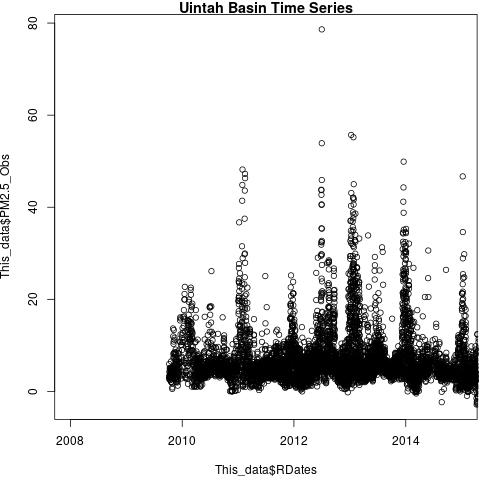
\includegraphics[width=0.77\textwidth]{Code_Outputs/UintahBasin_time_series.jpg} 
\caption{\label{fig:UintahBasinTS}Uintah Basin time series. There are 0 data points (out of 27330) with concentrations greater than 200 ug/m3} 
\end{figure} 
 

\begin{figure} 
\centering 
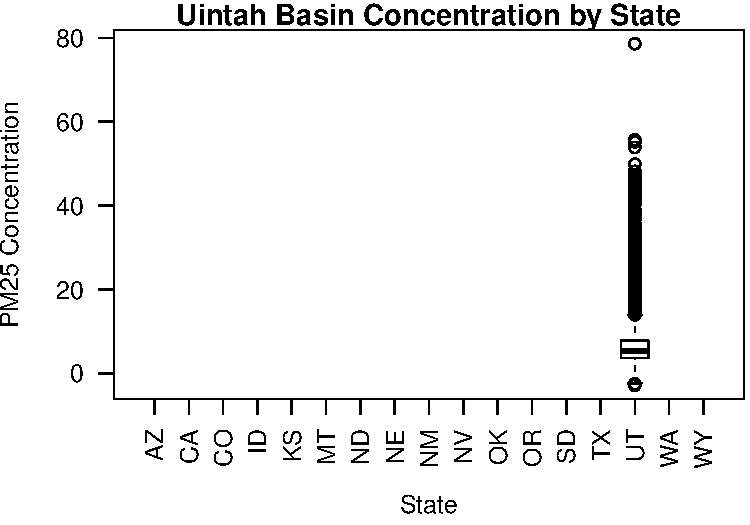
\includegraphics[width=0.77\textwidth]{Code_Outputs/UintahBasin_state_boxplots.pdf} 
\caption{\label{fig:UintahBasinBP}Uintah Basin box plots.} 
\end{figure} 
 

\begin{figure} 
\centering 
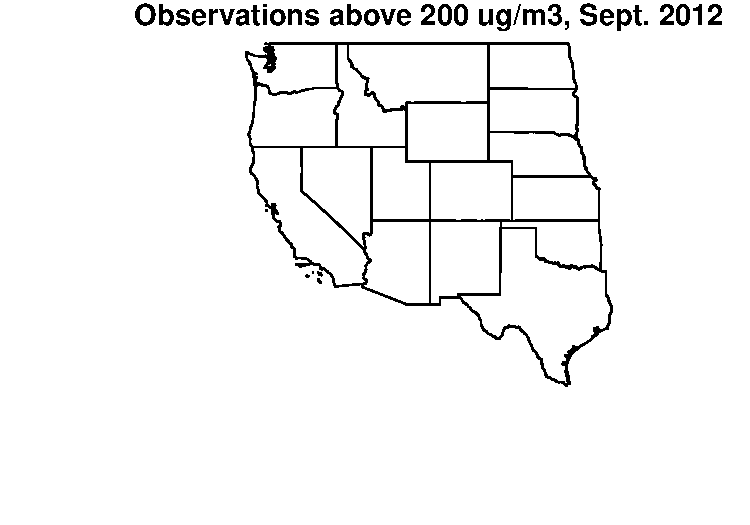
\includegraphics[width=0.77\textwidth]{Code_Outputs/UintahBasinSep2012High_map.pdf} 
\caption{\label{fig:UintahBasinS12}Uintah Basin map of locations with PM2.5 above 200 ug/m3 during Sept 2012.} 
\end{figure} 
 
